
% tipo de documento
\documentclass{article}

% formato de página
\usepackage[margin=1.5cm, letterpaper]{geometry}

% idioma de los macros
\usepackage[spanish]{babel}
\usepackage[utf8]{inputenc}

% vínculos
\usepackage{hyperref}

% manejo de ecuaciones
\usepackage{amsmath}

% manejo de figuras
\usepackage{graphicx}
\graphicspath{ {./img_fig/} }
\usepackage{float}

% texto del documento
\begin{document}
    \title{
        Organización y Arquitectura de Computadoras \\
        Práctica 7: Convención de llamadas a subrutinas \\
    }
    \date{
        14 de abril del 2019
    }
    \author{
        Sandra del Mar Soto Corderi \\
        Edgar Quiroz Castañeda
    }
    \maketitle

    \section{Preguntas}
    \begin{enumerate}
    
    %1
    \item {
    ¿Qué utilidad tiene el registro $\textbf{\$fp}$? ¿Se puede prescindir de el?\\
	El registro $\textbf{\$fp}$ es el que corresponde al Apuntador del marco, 
	el cual guarda la dirección de la última palabra del marco. \\
	Un apuntador de marco, si es utilizado, apunta a una dirección en la pila 
	donde los argumentos y variables locales para una función(subrutina) 
	invocada son localizadas. \\
	Este apuntador es establecido en la entrada de una función y se mantiene 
	constante en la ejecución de la función invocada.\\
	Sí se puede prescindir del fp, siempre y cuando se sepa exactamente la
	cantidad de valores que se deben guardar en cada marco, esto es que no haya
	una cantidad variable de variables necesarias para una rutina dada. \\
	No todos los procesadores tienen los recursos de hardware para implementar 
	un apuntador de marco y algunas implementaciones donde se sabe exactamente 
	la distancia del marco, no quieren tener la sobrecarga adicional de 
	mantenerlo.
	}
	%2
	\item {
	Definimos como \textbf{subrutina nodo} a una subrutina que realiza una o más
	invocaciones a otras subrutinas y como \textbf{subrutina hoja} a una subrutina
	que no realiza llamadas a otras subrutinas. \\
	Notemos que dada una rutina arbitraria, su marco debe tener al menos los
	cuatro espacios para los argumentos según el protocolo dado.\\
	Entonces, a lo menos, el marco tendría un tamaño de 16 bytes, que pasaría
	cuando no tenga que almacenar nada de su invocador ni de sus invocados y
	tampoco requiera una cantidad variable de variables locales que necesite
	guardar entre llamados a subrutinas.
	
		\begin{enumerate}
			%a
			\item {
			¿Cuál es el tamaño mínimo que puede tener un marco para una 
			subrutina nodo? ¿Bajo qué condiciones ocurre?\\
			Sólo se guardan cosas en el marco durante el preámbulo y la 
			invocación.\\
			Para que una rutina llame a otra, durante su preámbulo debe guardar 
			su dirección de retorno en su marco, pues al invocar a otras rutinas
			éste será modificado. Además, debe almacenar los registros
			almacenados($\$si$) que se vayan a modificar durante su ejecución.\\
			En el caso extremo, digamos que no modifica ninguno.\\
			Durante la invocación, la única modificación que debe hacer al marco
			es guardar los registros temporales si los va a necesitar después.
			En el caso extremo digamos que no los necesita, entonces el marco 
			no se modificaría al hacer durante las invocaciones.\\
			Entonces el tamaño mínimo del marco es el tamaño mínimo de cuaquier
			rutina más el registro para guardar su dirección de retorno, que 
			sería 20 bytes en total, que sería 24 bytes con relleno.\\
			Y esto ocurriría cuando no necesite guardar ningún registro temporal
			entre llamadas a subrutinas y no utilice registros almacenados.
			}
			%b
			\item {
			¿Cuál es el tamaño mínimo que puede tener un marco para una 
			subrutina hoja? ¿Bajo qué condiciones ocurre?\\
			Sólo se guardan cosas en el marco durante el preámbulo y la 
			invocación.\\
			Cómo no una subrutina hoja no hace llamadas a otras rutinas, nunca 
			habría una invocación.\\
			En cuanto al preámbulo, tenemos que, como no hay llamadas a
			subrutinas, no es necesario guardar la dirección de retorno.\\
			Entonces sólo sería necesario guardar los registros almaccenas que 
			se vayan a modificar durante la ejecución de esa rutina.\\
			En el caso extremo, digamos que no se usan registras almacenados.\\
			Entonces, el tamaño mínimo del marco sería el mínimo de cualquier
			subrutina arbitraria, que es 16 bytes.\\
			Y este caso se daría cuando no se usen registros almacenados en la
			subrutina hoja.
			}
		\end{enumerate}
		
	
	}
	
		
	%3
	\item{
	Considera el siguiente pseudocódigo de la figura 3. En donde a[5] es un
	arreglo de tamaño 5 y “...” son otras acciones que realiza la rutina, además
	, supón que en la función B se realizan cambios en los registros $\$s0,
	\$s1$ y $\$s2$. Bosqueja la pila de marcos después del preámbulo de la 
	función B.
	
	\begin{figure}[H]
		\centering
		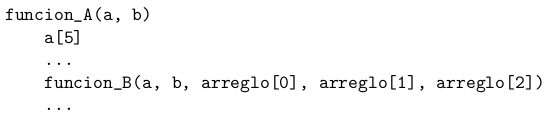
\includegraphics[scale=0.5]{Figura1.png}
		\caption{Rutina con llamado a subrutina}
	\end{figure}

	La pila sería, en el caso general,
	
	\begin{figure}[H]
		\centering
		\includegraphics[scale=0.5]{Figura2.png}
		\caption{Pila de marcos de la función B}
	\end{figure}
	}
	Con $\texttt{\$a0 = a}$, $\texttt{\$a1 = b}$, $\texttt{\$a2 = arreglo[0]}$,
	$\texttt{\$a3 = arreglo[1]}$ y $\texttt{\$a4 = arreglo[2]}$.\\
	La existencia de $\texttt{\$ra}$ en el marco de $\texttt{funcion\_B}$
	dependería de si esa función llama a otras subrutinas o no.\\
	En cuanto a los valores de $\texttt{a[]}$, nunca se especifica dónde se
	guardan, así que en el caso general pueden estar bien en los registros 
	temporales de la $\texttt{funcion\_A}$ o en los registros almacenados del
	marco de $\texttt{funcion\_B}$, dependiendo de como se implemente la 
	$\texttt{funcion\_A}$ o en ninguna parte si no son necesarios después de la
	llamada a la $\texttt{funcion\_B}$.
    \end{enumerate}
\end{document}